\documentclass[a4paper, 12pt]{article}

%%% Работа с русским языком
\usepackage{cmap}					% поиск в PDF
\usepackage{mathtext} 				% русские буквы в формулах
\usepackage[T2A]{fontenc}			% кодировка
\usepackage[utf8]{inputenc}			% кодировка исходного текста
\usepackage[russian]{babel}	% локализация и переносы

%%% Дополнительная работа с математикой
\usepackage{amsmath,amsfonts,amssymb,amsthm,mathtools} % AMS
\usepackage{icomma} % "Умная" запятая: $0,2$ --- число, $0, 2$ --- перечисление

%% Номера формул
%\mathtoolsset{showonlyrefs=true} % Показывать номера только у тех формул, на которые есть \eqref{} в тексте.

%% Шрифты
\usepackage{euscript}	 % Шрифт Евклид
\usepackage{mathrsfs} % Красивый матшрифт

%% Поля
\usepackage[left=2cm,right=2cm,top=2cm,bottom=2cm,bindingoffset=0cm]{geometry}

%% Русские списки
\usepackage{enumitem}
\makeatletter
\AddEnumerateCounter{\asbuk}{\russian@alph}{щ}
\makeatother

%%% Работа с картинками
\usepackage{graphicx}  % Для вставки рисунков
\graphicspath{{images/}{images2/}}  % папки с картинками
\setlength\fboxsep{3pt} % Отступ рамки \fbox{} от рисунка
\setlength\fboxrule{1pt} % Толщина линий рамки \fbox{}
\usepackage{wrapfig} % Обтекание рисунков и таблиц текстом

%%% Работа с таблицами
\usepackage{array,tabularx,tabulary,booktabs} % Дополнительная работа с таблицами
\usepackage{longtable}  % Длинные таблицы
\usepackage{multirow} % Слияние строк в таблице

%% Красная строка
\setlength{\parindent}{2em}

%% Интервалы
\linespread{1}
\usepackage{multirow}

%% TikZ
\usepackage{tikz}
\usetikzlibrary{graphs,graphs.standard}

%% Верхний колонтитул
\usepackage{fancyhdr}
\pagestyle{fancy}

%% Перенос знаков в формулах (по Львовскому)
\newcommand*{\hm}[1]{#1\nobreak\discretionary{}
	{\hbox{$\mathsurround=0pt #1$}}{}}

%% Мои дополнения
\usepackage{float} %Добавляет возможность работы с командой [H] которая улучшает расположение на странице
\usepackage{gensymb} %Красивые градусы
\usepackage{graphicx}               % Импорт изображений
\usepackage{caption} % Пакет для подписей к рисункам, в частности, для работы caption*

% подключаем hyperref (для ссылок внутри  pdf)
\usepackage[unicode, pdftex]{hyperref}

%%% Теоремы
\theoremstyle{plain}                    % Это стиль по умолчанию, его можно не переопределять.
\renewcommand\qedsymbol{$\blacksquare$} % переопределение символа завершения доказательства

\newtheorem{theorem}{Теорема}[section] % Теорема (счетчик по секиям)
\newtheorem{proposition}{Утверждение}[section] % Утверждение (счетчик по секиям)
\newtheorem{definition}{Определение}[section] % Определение (счетчик по секиям)
\newtheorem{corollary}{Следствие}[theorem] % Следстиве (счетчик по теоремам)
\newtheorem{problem}{Задача}[section] % Задача (счетчик по секиям)
\newtheorem*{remark}{Примечание} % Примечание (можно переопределить, как Замечание)
\newtheorem{lemma}{Лемма}[section] % Лемма (счетчик по секиям)

\begin{document}
	\newcommand{\HRule}{\rule{\linewidth}{0.7mm}} % Defines a new command for the horizontal lines, change thickness here
	
	\begin{center}
		\large\textbf{Московский Физико-Технический Институт}\\ % Name of your university/college
		\large\textbf{(государственный университет)}
	
		\vfill
		
		\Large Лабораторная работа по курсу общей физики № *labnum*\\[0.5cm] % Preambule of your document title
		
		
		\HRule
		\\[0.4cm]
		{ \huge \bfseries *name of your labwork*}% Title of your document
		\\[0.4cm] 
		\HRule
		\\[0.5cm]
		
		\ \\
	\textbf{\large Автор:} \\	
	\large *your name* *groupname*\\ % Your name and something more, your group num for example
		\vfill
		\hspace*{-0.8 cm}
\includegraphics[width=100 pt]{frkt_logo}\\ % logo of your  company/university/college
		\large Долгопрудный, 2021 % location and year
	\end{center}

\newpage
\setcounter{page}{2}
\fancyfoot[c]{\thepage}
\fancyhead[L] {Работа № *labnum*} % some information in page header
\fancyhead[R]{}
	
	\section*{Теоретическая справка}
	\subsection*{Определение фокусных расстояний положительных и отрицательных линз и положений главных плоскостей сложной оптической системы}
	
	Оптическую систему называют \textbf{центрированной}, если центры всех поверхностей лежат на одной прямой, которую называют \textbf{главной оптической осью системы}. 
	
	Световые пучки называются \textbf{гомоцентрическими}, если, выйдя из одной точки и пройдя оптическую систему, пучки или их продолжения снова сходятся в одной точке.
	
	Идеальной оптической системой называют систему, в которой сохраняется \textbf{гомоцентричность} пучков и изображение геометрически подобно
	предмету
	
	Общий вид сложной оптической системы изображен на рис. \ref{fig:optical_system}.
	
	\begin{wrapfigure}{l}{0.45\textwidth}
		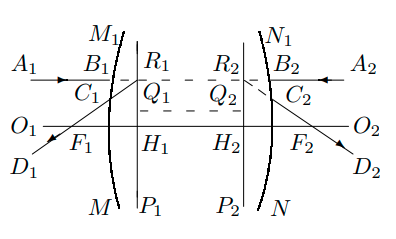
\includegraphics[width = 0.45\textwidth]{images/optical_system.png}
		\caption{сложная оптическая система}
		\label{fig:optical_system}
	\end{wrapfigure}

	Пусть $MM_1$ и $NN_1$ -- крайние поверхности, ограничивающие оптическую систему, а $O_1O_2$ -- главная оптическая ось. Точку $F_2$ называют \textbf{задним фокусом системы} (фокусом в пространстве изображений). Плоскость, перпендикулярная $O_1O_2$ и проходящая
	через точку $F_2$, называется \textbf{задней фокальной плоскостью}. Точку $F_1$ называют \textbf{передним фокусом системы} (фокусом в пространстве предметов). 
	
	Продолжим теперь $C_1D_1$ и $C_2D_2$ до пересечения с продолжениями $A_1B_1$ и $A_2B_2$ и отметим точки пересечения $R_1$ и $R_2$. Плоскости $P_1$ и $P_2$ называются \textbf{главными плоскостями}, а точки $H_1$ и $H_2$ -- \textbf{главными точками системы}. Расстояния от главных точек до фокусов называются \textbf{фокусными расстояниями}: $f_1 = H_1F+1$, $f_2 = H_2F_2$. В том случае, когда с обеих сторон системы находится одна и та же среда (например, воздух), $f_1 = f_2 = f$.
	
	\begin{wrapfigure}{r}{0.45\textwidth}
		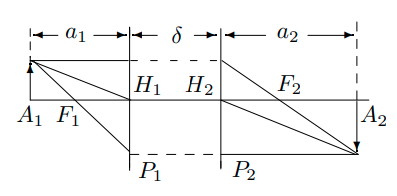
\includegraphics[width = 0.45\textwidth]{images/image_in_thick_lense.png}
		\caption{Построение изображения в сложной оптической системе}
		\label{fig:image_in_thick_lense}
	\end{wrapfigure}

	Соотношения между величинами при построении изображения в толстой линзе удовлетворяют уравнению:
	
	\begin{equation} \label{eq:thin_lense_eq}
		\frac{1}{a_1} + \frac{1}{a_2} = \frac{1}{f}
	\end{equation}
	
	\subsubsection*{Способы определения фокусного расстояния тонкой положительной линзы}
	
	\begin{enumerate}
		\item Исходя из формулы тонкой линзы \eqref{eq:thin_lense_eq}, полагая $\delta = 0$.
		
		\item Пусть расстояние между предметом и экраном превышает $4f$. При этом всегда найдутся два таких положения линзы, при которых на экране получаются отчётливые изображения предмета (в одном случае уменьшенное, в другом -- увеличенное).
		
		\begin{figure}
			\centering
			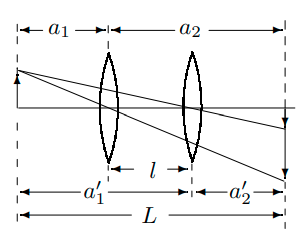
\includegraphics[scale=0.5]{images/second_method.png}
			\caption{Нахождение фокусов тонкой собирающей линзы}
			\label{fig:second_method}
		\end{figure}
	
		Из соображений симметрии $a_1 = a_2'$ и $a_1' = a_2$. Тогда путем математических преобразований можно получить:
		
		\[ a_1 = \frac{L - l}{2}; ~~ a_2 = \frac{L + l}{2} \Rightarrow \]
		
		откуда с помощью \eqref{eq:thin_lense_eq} получаем:
		
		\begin{equation} \label{eq:second_method}
			f = \frac{L^2 - l^2}{4L}
		\end{equation}
		
		\item Фокусное расстояние тонкой положительной линзы можно определить с помощью зрительной трубы, настроенной на бесконечность, то есть на параллельный пучок лучей.
	\end{enumerate}

	\subsubsection*{Способы определения фокусного расстояния тонкой отрицательной линзы}
	
	\begin{enumerate}
		\item С помощью вспомогательной собирающей линзы получаем действительное изображение и используем формулу тонкой линзы.
		
		\begin{figure}
			\centering
			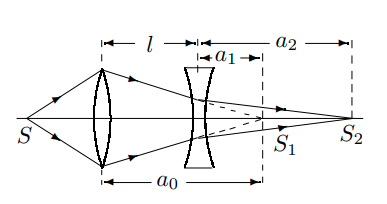
\includegraphics[width = 0.45\textwidth]{images/image_in_negative_lense.png}
			\caption{Изображение в рассеивающей линзе}
			\label{fig:image_in_negative_lense.png}
		\end{figure}
	
		\item С помощью зрительной трубы, установленной на бесконечность.
	\end{enumerate}

	\subsection*{Определение фокусного расстояния и положения главных плоскостей сложной оптической системы}
	
	Фокусное расстояние толстой положительной линзы определяют по методу Аббе рис. \ref{fig:Abbe_method}.
	
	\begin{figure}
		\centering
		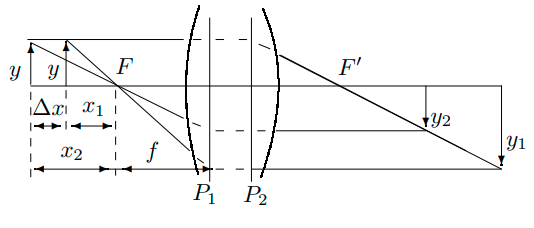
\includegraphics[scale=0.5]{images/Abbe_method.png}
		\caption{метод Аббе}
		\label{fig:Abbe_method}
	\end{figure}

	Линейные увеличения для разных положений объекта:
	
	\[ \Gamma_1 = \frac{y_1}{y} = \frac{f}{x_1}; ~~ \Gamma_2 = \frac{y_2}{y} = \frac{f}{x_2} \]
	
	тогда нетрудно получить соотношение:
	
	\begin{equation} \label{eq:thik_lense_focus}
		f = \frac{\Delta x}{1 / \Gamma_1 - 1 / \Gamma_2}
	\end{equation}
	
	Для нахождения главных плоскостей системы недостаточно знать фокусное расстояние, нужно определить ещё положения главных фокусов. Это можно сделать при помощи зрительной трубы, настроенной на бесконечность.
	
	Теоретически фокусное расстояние $f_0$ сложной системы, состоящей из двух тонких положительных линз, можно рассчитать, если известны фокусные расстояния каждой линзы и расстояние между их центрами $l_{12}$:
	
	\begin{equation} \label{eq:theoretical_thik_lense_focus}
		\frac{1}{f_0} = \frac{1}{f_1} + \frac{1}{f_2} - \frac{|l_{12}|}{f_1 f_2}
	\end{equation}
	
	\subsection*{Недостатки (аберрации) реальных оптических систем}
	
	В идеальных оптических системах лучи, вышедшие из одной точки объекта, пересекаются в одной и той же точке изображения независимо от угла испускания и от длины волны света. В реальных системах -- из-за несовершенства линз -- такая зависимость наблюдается. Основными погрешностями линз являются сферическая и хроматическая аберрации.
	
	\subsection*{Сферическая аберрация}
	
	Сферическая аберрация возникает при преломлении широких (не параксиальных) пучков свет а на сферических поверхностях линз.
	
	\begin{wrapfigure}{l}{0.45\textwidth}
		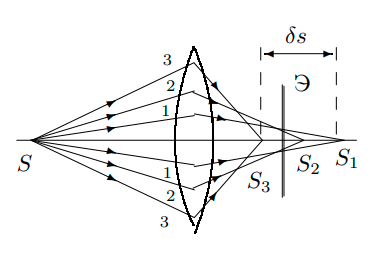
\includegraphics[width = 0.45\textwidth]{images/spherical_aberration.png}
		\caption{Сферическая аберрация}
		\label{fig:spherical_aberration}
	\end{wrapfigure}

	Сферическую аберрацию характеризуют с помощью так называемой \textbf{продольной аберрации} $\delta s$ равной расстоянию между точками пересечения крайних и центральных лучей с главной оптической осью.
	
	Для лучей, проходящих на расстоянии $h$ от центра линзы, расстояние $s$ выражается соотношением:
	
	\begin{equation}
		s(h) = \frac{R}{n - 1} \left(1 - \frac{n^2 h^2}{2 R^2} \right)
	\end{equation}
	
	\begin{wrapfigure}{r}{0.45\textwidth}
		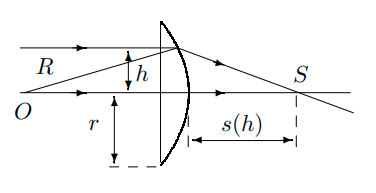
\includegraphics[width = 0.45\textwidth]{images/aberation_equation.png}
		\caption{Сферическая аберрация плосковыпуклой линзы}
		\label{fig:aberration_equation}
	\end{wrapfigure}

\end{document}